\documentclass[10pt,a4paper]{article}
\usepackage[margin=2.4cm,top=2.2cm,bottom=2.4cm]{geometry}
\usepackage{booktabs,longtable,multirow,array}
\usepackage{graphicx,caption,subcaption,float}
\usepackage{amsmath,amssymb}
\usepackage[table]{xcolor}
\usepackage{microtype,enumitem}
\usepackage[numbers,sort&compress]{natbib}
\usepackage[hidelinks,breaklinks]{hyperref}

\definecolor{ink}{HTML}{1A1A1A}
\definecolor{accent}{HTML}{1B5E8F}
\definecolor{warm}{HTML}{B5502A}
\definecolor{rule}{HTML}{D4D0C8}
\definecolor{panel}{HTML}{F6F4F0}

\captionsetup{font=small,labelfont={bf,color=accent},skip=4pt,justification=raggedright,singlelinecheck=false}
\captionsetup[sub]{font=small}
\setlist[itemize]{leftmargin=1.1em,itemsep=1pt,topsep=3pt,parsep=0pt}
\setlist[enumerate]{leftmargin=1.4em,itemsep=1pt,topsep=3pt,parsep=0pt}
\renewcommand{\arraystretch}{1.12}
\setlength{\tabcolsep}{4.5pt}

% a boxed aside, used for epistemic-status and caveat panels
% a colour-boxed aside. \colorbox grabs its argument as a box, so it cannot be split
% across the environment's begin/end -- the content is captured in an lrbox first.
\newsavebox{\asidebox}
\setlength{\fboxsep}{7pt}
\newenvironment{aside}[1]{%
  \par\medskip\noindent
  \begin{lrbox}{\asidebox}%
  \begin{minipage}{\dimexpr\linewidth-2\fboxsep\relax}%
  \small\textbf{\textcolor{accent}{#1}}\par\smallskip\small
}{%
  \end{minipage}%
  \end{lrbox}%
  \noindent\colorbox{panel}{\usebox{\asidebox}}\par\medskip
}

% axis identifiers
\newcommand{\ax}[1]{\textcolor{accent}{\textbf{#1}}}
\newcommand{\bx}[1]{\textcolor{warm}{\textbf{#1}}}
\newcommand{\mx}[1]{\textbf{#1}}
\newcommand{\trend}[1]{\medskip\noindent\textbf{#1}\quad}
% verdict tags for the novelty table
\newcommand{\vrep}{\textsc{replication}}
\newcommand{\vext}{\textsc{extension}}
\newcommand{\vnov}{\textcolor{warm}{\textsc{novel}}}
\newcommand{\vcon}{\textcolor{warm}{\textsc{contradicts}}}

\title{\vspace{-1.4cm}\textbf{A Scaffolding Atlas}\\[2pt]
\large How agent-system configuration reshapes model behaviour, and what changes inside the model\\[2pt]
\normalsize\normalfont Exploratory findings from \texttt{study\_v4} --- 1{,}332 cells, 10{,}714 episodes, 61.6\,EFLOP, Qwen3 4B--32B}
\author{}
\date{\small 7 September 2026}

\begin{document}
\maketitle
\vspace{-1.1cm}

\begin{abstract}
\noindent We ran a factorial study of multi-agent inference on one model family and two benchmarks, varying routing topology, team size, interaction depth, compute allowance, model scale, prompt framing and aggregation rule, and captured the residual stream of the flagship model during the runs. This atlas organises what came out into three taxonomies --- configuration axes, behaviour axes, mechanistic observables --- and then works through the relations between them. The confirmatory analysis rejected nothing; this document is about the conditional structure underneath that null. Three findings organise the rest. First, benchmark difficulty is bimodal and gates every other axis: 55\% of items are solved by no configuration and 19\% by all, so the entire orchestration effect lives in the 11\% in between, where the spread between topologies is 0.156 against 0.040 pooled. Second, every mechanism the system uses to convert samples into an answer --- plurality voting, an LLM judge, stated confidence, a self-forecast --- reads a signal that encodes item difficulty and mainstream-ness but not correctness, so pass@$k$ climbs while vote@$k$ stays flat and the generation--verification gap widens with every sample. Third, peer exposure reshapes the geometry of the committed answer state: variance concentrates from 61\% to 74\% on a single axis while the mean separation between agents is unchanged, which is anisotropy rather than the convergence it is easy to mistake it for. We assess 34 claims against the literature under adversarial adjudication: none survives as novel --- 16 replicate, 16 extend known results into a new regime, and 2 contradict prior work --- so the contribution is the controlled design and several specific new measurements, not new phenomena. We close with the eleven relations most worth instrumenting next.
\end{abstract}

\begin{aside}{Epistemic status --- read this first}
Everything here is \textbf{exploratory and uncorrected}. The pre-registered confirmatory analysis of this run rejected no hypothesis family under Holm correction; the intervals quoted below are percentile bootstraps reported as effect sizes, not tests, and no multiplicity adjustment is applied anywhere. Numbers are recomputed from the sealed tables, item files and activation store by the scripts in \texttt{scripts/}; nothing is transcribed from an intermediate report. Scope limits that apply to every statement: one model family (Qwen3 dense, 4B--32B), one frozen sampling recipe, two benchmarks, a self-judged exam metric, and \textbf{correlational} mechanism only --- the causal half of the neural design (activation edits, donors, specificity controls) was cut before dispatch and is recorded as amendment R1. Where a claim rests on few items, or was overturned or narrowed by an adversarial re-derivation, it says so inline.
\end{aside}

\section{How to read this atlas}

The document separates three things that are usually collapsed. A \textbf{configuration axis} (\ax{C1}--\ax{C10}) is something an engineer chooses when building an agent system. A \textbf{behaviour axis} (\bx{B1}--\bx{B8}) is something the assembled system does that we can measure from its outputs. A \textbf{mechanistic observable} (\mx{M1}--\mx{M9}) is a property of the model's internal state while it does it. Part~\ref{part:tax} defines all three, with the realised levels and the sample size behind each. Part~\ref{part:trends} then works through configuration~$\to$~behaviour (\S\ref{sec:cb}), configuration~$\to$~mechanism (\S\ref{sec:cm}), mechanism~$\to$~behaviour (\S\ref{sec:mb}), and what can and cannot be said about mediation (\S\ref{sec:med}). Part~\ref{part:pos} places each finding against the literature and ranks what to do next.

Trends are labelled by the pair they connect, so \ax{C1}$\times$\bx{B5} is ``routing topology affects calibration''. Each carries a status: \textsc{confirmed} (independently re-derived through a different join), \textsc{narrowed} (re-derivation changed the claim), or \textsc{unverified} (computed once). \textbf{Null results are reported as findings}, not omitted --- an atlas that says which knobs do nothing is as useful as one that says which do, and \S\ref{sec:nulls} collects them.

\begin{aside}{One methodological warning that this study learned the hard way}
Scale-free and scale-carrying geometry metrics dissociate. The headline mechanistic result was first written up as agents' internal states ``converging'' under peer exposure, on the strength of a participation-ratio drop. The mean distance between those states is in fact unchanged (\S\ref{sec:cm}); the metric had moved because the \emph{shape} of the spread changed, not its size. Any claim in this document that rests on one family of metric is reported beside the other.
\end{aside}

\section{The experiment in one page}\label{sec:exp}

A frozen generation pipeline ran 1{,}332 cells (10{,}714 episodes, 338{,}969 requests, 61.6\,EFLOP) over 400 main items --- 200 HLE-Verified text-only exam questions and 200 BigCodeBench programming tasks --- plus a 20-item development split. All solver calls on all checkpoints share one sampling recipe (temperature 0.6, top-$p$ 0.95, top-$k$ 20, thinking on, 8{,}192-token output cap); selectors, judges and forecasters run thinking-off at temperature 0. Answers are content-addressed, so an identical request anywhere in the design is served from store rather than regenerated --- a fact with consequences in \S\ref{sec:nominal}.

Eight modules cross the axes: \textbf{F} independent 10-draw banks under a $2\times2$ framing manipulation; \textbf{A} the five routing topologies at fixed team size and budget; \textbf{N} team size $\in\{1,2,3,5,9\}$ plus two one-round controls; \textbf{D} consumer degree $\in\{0,1,2,4,8\}$; \textbf{E} six repeated episodes per configuration; \textbf{M} the dense checkpoint panel 4B/8B/14B; \textbf{MX} scale crossed with team size and budget; \textbf{B} the budget panel. Selection is sealed before evaluation: candidate pools are frozen and hashed, then a plurality vote and a pointwise LLM judge are applied, then correctness is joined. Exam answers are graded by Qwen3-32B itself using the official judge prompt; code is executed in a sandboxed container.

Separately, a measurement-only capture replayed stored token sequences through an HF-transformers copy of the flagship and read the residual stream at blocks 15, 31 and 47 of 64, at five structural anchors from the prompt to the token closing the answer object. Parity is exact: byte-identical re-tokenisation on every replayed completion, zero identity failures, and a two-pass logit discrepancy of 0.0.

\section{Global caveats}\label{sec:caveats}

\begin{itemize}
\item \textbf{The exam benchmark is at floor.} 141 of 200 HLE items are never solved in ten neutral draws (code: 80 of 200). Within HLE this concentrates in exact-match Gold items (84\% never solved). Most exam contrasts are therefore bounded by a handful of items and several are not identifiable at all.
\item \textbf{The judge is the solver.} Exam correctness is adjudicated by the same checkpoint that produced the answers. The planned audit --- a multiple-choice-based false-positive/negative bound and a 100-candidate human sample --- \textbf{was never produced}; the code exists but no artifact does. Absolute exam accuracies should be read as judge-agreement rates.
\item \textbf{Code ``voting'' is syntactic.} Candidate programs are grouped by AST canonicalisation with an exact-source fallback. Equivalent programs written differently do not group. Verified consequence: grouping errs only by splitting --- in 800 pools not one vote class ever merged a correct and an incorrect program.
\item \textbf{Truncation is an outcome.} With one 8{,}192-token budget for thinking plus answer, a long reasoning trace yields no parseable answer and is scored incorrect. Across 348{,}377 candidates the valid fraction is 0.840, and 46{,}485 failures are truncations.
\item \textbf{Module D lost its entire code half.} 500 sealed degree selections on BigCodeBench were never evaluated; the degree module is exam-only on 50 items. Module E has no rank-prefix panel (15 items per domain).
\item \textbf{The activation capture is partial.} 7{,}278 of 10{,}063 planned work items were captured. Geometry exists for 293 hub items, 240 peer-revision items and only 124 independent-sampling items, and \textbf{no decentralised root group has its contracted five states} --- so there is no within-episode before/after comparison anywhere in the data.
\end{itemize}

\part{The three taxonomies}\label{part:tax}

\section{Configuration axes}\label{sec:config}

\begin{table}[H]\centering\small
\caption{Configuration axes as realised. ``Panel'' is the item count the axis was varied on; the flagship panel is 400 items. An axis is only an axis where the levels produced different episodes --- see \S\ref{sec:nominal}.}
\label{tab:config}
\begin{tabular}{@{}llp{5.6cm}rl@{}}
\toprule
& Axis & Realised levels & Panel & Module \\
\midrule
\ax{C1} & Routing topology & stateless-fresh, stateless-with-history, independent+vote, decentralised peer revision, centralised hub--worker & 400 & A \\
& \quad controls & one-round revision, private (no-peer) revision & 100 & N \\
\ax{C2} & Team size $N$ & 1, 2, 3, 5, 9 & 100 & N, MX \\
\ax{C3} & Interaction depth & revision rounds 1--8; hub cycles 1--8; consumer degree 0, 1, 2, 4, 8 & 400 / 50 & A, D \\
\ax{C4} & Compute allowance & $B_1{=}B_0$, $B_2{=}2B_0$, $B_4{=}4B_0$ with $B_0\,{=}\,11.97$\,PFLOP; hard caps 64 solver calls, 8{,}192 output tokens, 8 rounds, 8 cycles & 100 & B, MX \\
\ax{C5} & Model scale & 4B, 8B, 14B, 32B (dense Qwen3, matched FLOP allowance) & 150 & M, MX \\
\ax{C6} & Prompt framing & team-frame $\times$ vote-aware $\in\{00,01,10,11\}$, plus a truthful native clause & 400 & F, A \\
\ax{C7} & Aggregation rule & plurality vote, pointwise LLM judge, policy-native synthesis & 400 & all \\
\ax{C8} & Repetition & 6 independent episodes of a fixed configuration & 30 & E \\
\midrule
\multicolumn{5}{@{}l}{\emph{Moderators promoted to first-class axes, because they gate everything above}}\\
\ax{C9} & Task domain \& format & exam (exact-match / multiple-choice; Gold / Revision strata) vs.\ code & 400 & all \\
\ax{C10} & Item difficulty band & never solved / hard / contested / easy, from the neutral 10-draw bank & 400 & derived \\
\bottomrule
\end{tabular}
\end{table}

\subsection{Nominal versus realised configuration}\label{sec:nominal}

Because generation is content-addressed, two nominally different cells that issue the same requests are the same episode. Grouping the 59 nominal (module, topology, checkpoint, $N$, budget) cells on a shared panel by their per-item outcome vectors, they collapse to \textbf{40 distinct correctness vectors and 43 distinct compute vectors}. The largest identical group has \textbf{seven} members: every independent-sampling cell at $N=1,2,3,5,9$ and two of the scale-crossing cells are byte-identical to stateless-fresh sampling, because the budget --- not $N$ --- determines how many samples are drawn, and the slot assignment is metadata. \emph{Team size is not a manipulable axis for independent sampling in this design.} Any analysis reading a trend across those levels is reading one number five times. The same applies to several budget contrasts (\S\ref{sec:budget}).

\section{Behaviour axes}\label{sec:behaviour}

\begin{table}[H]\centering\small
\caption{Behaviour axes. ``Pool'' means the sealed set of candidates a selector chose from; ``episode'' means one run of a configuration on one item.}
\label{tab:behaviour}
\begin{tabular}{@{}llp{9.4cm}@{}}
\toprule
& Axis & Definition as measured \\
\midrule
\bx{B1} & Task accuracy & correctness of the answer the system actually delivers (policy-native final, or the selector's pick). A missing or unparseable final is scored incorrect. \\
\bx{B2} & Pool quality & mean per-opportunity correctness (invalid candidates count as wrong, in the denominator); oracle coverage $=$ the pool contains at least one correct answer; pass@$k$ by the unbiased finite-sample estimator. \\
\bx{B3} & Selection efficiency & oracle coverage minus delivered accuracy (the ``selection gap''); vote@$k$ and judge@$k$ over the same prefixes; the winning class's share of the pool. \\
\bx{B4} & Consensus \& diversity & agreement (winning class $\div$ valid candidates); unanimity; all-singleton rate; tied classes; per-round answer switching. \\
\bx{B5} & Calibration & stated confidence; Brier; bias $E[q-y]$; resolution (confidence given correct minus given wrong); reliability bins; the separate self-forecast channels. \\
\bx{B6} & Resource behaviour & calls admitted; realised FLOPs as a fraction of the allowance; which cap terminated the episode; truncation rate. \\
\bx{B7} & Format validity & fraction of candidates that parse; failure codes (truncated, schema, not-JSON). \\
\bx{B8} & Stability & spread of the same configuration's accuracy across independent repeats, and within-item variance. \\
\bottomrule
\end{tabular}
\end{table}

\section{Mechanistic observables}\label{sec:mech}

Comparable states are the $s=5$ residual vectors of an item's five agents at one anchor and block. Independent-sampling groups draw 5 of $\approx58$ available states, hash-seeded, averaged over 100 subsamples; peer-revision groups have exactly 5. All figures below are recomputed from the raw \texttt{fp16} vectors, not the shipped geometry table, which carries a defective agreement column (Appendix~\ref{app:defects}).

\begin{table}[H]\centering\small
\caption{Mechanistic observables. The split between scale-free and scale-carrying families is the important one: they dissociate, and reading only one produced a wrong conclusion in this study.}
\label{tab:mech}
\begin{tabular}{@{}llp{8.6cm}@{}}
\toprule
& Observable & What it measures \\
\midrule
\mx{M1} & Scale-free spread & participation ratio $(\sum\lambda)^2/\sum\lambda^2$ and entropy effective rank of the covariance spectrum: \emph{how many directions} the five states vary along. Ceiling $\min(d_{\text{eff}},s-1)=4$. \\
\mx{M2} & Scale-carrying spread & mean, minimum and maximum pairwise Euclidean distance; total variance: \emph{how far apart} the states actually are. \\
\mx{M3} & Norm & mean $\lVert h\rVert$ of the state. \\
\mx{M4} & Angular dispersion & mean pairwise cosine distance on unit-normalised states. \\
\mx{M5} & Trajectory position & anchor $\in$ \{prompt, 32, 128, 512 generated tokens, token closing the answer object\}. \\
\mx{M6} & Depth & block 15, 31, 47 of 64 (quarter, half, three-quarter depth), residual stream after the block. \\
\mx{M7} & Linear decodability & item-grouped cross-validated probes for: which topology produced a report, item difficulty, candidate correctness (pooled and \emph{within item}), majority membership, the stated confidence value. \\
\mx{M8} & Displacement geometry & the vector between two conditions' mean states, and its alignment with a fitted axis against a spectrum-matched null. \\
\mx{M9} & Reader displacement & $\lVert h_{\text{report}}-h_{\text{task}}\rVert$ relative to $\lVert h_{\text{task}}\rVert$: how far a compiled handoff report moves a reader model's state. \\
\bottomrule
\end{tabular}
\end{table}

\part{Trends}\label{part:trends}

\section{Configuration \texorpdfstring{$\to$}{->} behaviour}\label{sec:cb}

\subsection{\ax{C10} gates every other axis}\label{sec:difficulty}

\trend{\ax{C10}$\times$\bx{B1} --- Orchestration only acts on a narrow band of items. \textsc{narrowed}}
Item difficulty, measured by an independent 10-draw bank under neutral framing, is bimodal: \textbf{221 of 400 items} are solved by no draw, \textbf{77} by nearly every draw, and only \textbf{45} sit in the contested band with single-draw success in $(0.3,0.7]$. Inside that band the five routing topologies span \textbf{0.156} (independent+vote 0.778 against the hub's 0.622, with a single draw at 0.540); pooled over all 400 items they span \textbf{0.040} (Table~\ref{tab:difficulty}, Figure~\ref{fig:difficulty}). The pooled number is the conditional effect diluted by three-quarters of a panel where nothing can move.

An adversarial re-derivation confirmed the bins and the contested-band lift (independent+vote gains $+0.239$ $[+0.12,+0.35]$ over a single draw, reproducing on both domains separately) but \textbf{narrowed the framing}: it is not true that \emph{every} effect lives in the contested band. In the easy band the two sequential policies genuinely gain over a single draw ($+0.051$ and $+0.064$), and the hub genuinely loses about ten points there (0.883 against stateless-with-history's 0.987). The correct statement is that the contested band is where topologies \emph{differentiate}, and the easy band is where a bad topology can still destroy value.

The never-solved band is not an artefact of ten draws. Across \textbf{3{,}613} flagship episodes on those items, \textbf{17} were ever solved at all, in 73 events. And difficulty manufactures a well-known pooled illusion: mean pairwise agreement between topologies on per-item correctness is $\phi=0.72$ pooled --- ``the policies solve the same items'' --- but $\phi=0.09$ inside the contested band, where they disagree almost completely.

\begin{figure}[H]\centering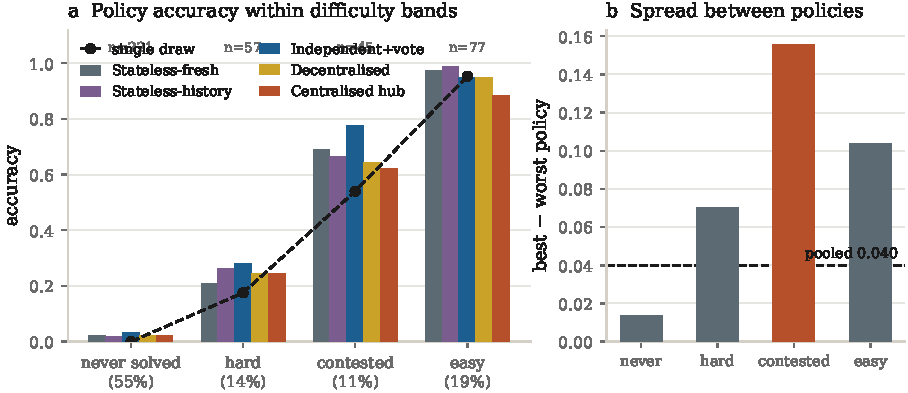
\includegraphics[width=\linewidth]{figures/f2_difficulty.pdf}
\caption{Difficulty gates orchestration. \textbf{(a)} Accuracy of the five topologies within each band, with the single-draw baseline. \textbf{(b)} The spread between best and worst topology is four times larger inside the contested band than pooled.}
\label{fig:difficulty}\end{figure}

\begin{tabular}{lcccc}
\toprule
& never solved & hard & contested & easy \\
items & 221 & 57 & 45 & 77 \\
single draw & 0.000 & 0.175 & 0.540 & 0.953 \\
\midrule
Stateless-fresh & 0.023 & 0.210 & 0.689 & 0.974 \\
Stateless-history & 0.018 & 0.263 & 0.667 & 0.987 \\
Independent+vote & 0.032 & 0.281 & 0.778 & 0.948 \\
Decentralised & 0.023 & 0.246 & 0.644 & 0.948 \\
Centralised hub & 0.023 & 0.246 & 0.622 & 0.883 \\
\midrule
best $-$ worst & 0.014 & 0.070 & \textbf{0.156} & 0.104 \\
\bottomrule
\end{tabular}
\vspace{-2pt}
\captionof{table}{\ax{C10}$\times$\bx{B1}: accuracy by routing topology within difficulty bands, 400 flagship items.}
\label{tab:difficulty}

\subsection{\ax{C1} routing topology}

\trend{\ax{C1}$\times$\bx{B1} --- Independent sampling with a vote is the best topology; the hub is the worst. \textsc{confirmed}}
At matched FLOP allowance (Table~\ref{tab:policies}, Figure~\ref{fig:policies}), independent+vote delivers 0.328 and the centralised hub 0.287, a paired difference of $+0.040$ $[+0.005,+0.078]$. The effect is carried by code ($+0.060$ $[+0.005,+0.115]$) and is not identifiable on the exam ($+0.020$ $[-0.025,+0.065]$), where a within-item permutation test on the five-topology ordering returns $P=0.72$ --- the exam panel cannot rank these policies at all. Peer revision, the most elaborate topology, sits mid-table at 0.302 and beats nothing reliably.

\trend{\ax{C1}$\times$\bx{B6} --- Four of five topologies hit a structural cap having spent a third of their compute. \textsc{confirmed}}
Independent sampling stops at the 64-call cap with 45\% of the FLOP allowance unspent; peer revision stops at the round cap at 30\%; the hub finishes voluntarily having used \textbf{1.9\%}. Only the smallest budget ever binds. This is the single most important fact about the design: \emph{the compute allowance is not what limits these systems, and therefore is not what differentiates them}.

\begin{figure}[H]\centering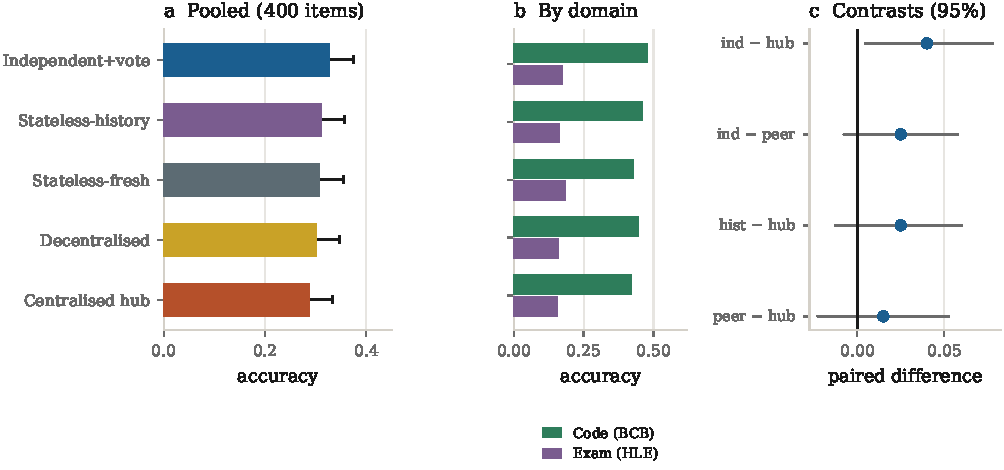
\includegraphics[width=\linewidth]{figures/f3_policies.pdf}
\caption{The five routing topologies at matched allowance. \textbf{(a)} Pooled accuracy with percentile intervals. \textbf{(b)} By domain --- the ordering is not stable across them. \textbf{(c)} Paired contrasts.}
\label{fig:policies}\end{figure}

\begin{tabular}{lccccrrlc}
\toprule
& \multicolumn{3}{c}{accuracy} & & \multicolumn{3}{c}{compute} & \\
\cmidrule(lr){2-4}\cmidrule(lr){6-8}
Routing topology & pooled & 95\% CI & exam & code & calls & spent & stop reason & conf. \\
\midrule
Independent+vote & 0.328 & [0.282, 0.375] & 0.175 & 0.480 & 64 & 0.451 & CALL\_CAP & 0.855 \\
Stateless-history & 0.312 & [0.268, 0.357] & 0.165 & 0.460 & 64 & 0.281 & CALL\_CAP & 0.937 \\
Stateless-fresh & 0.307 & [0.263, 0.355] & 0.185 & 0.430 & 64 & 0.418 & CALL\_CAP & 0.890 \\
Decentralised & 0.302 & [0.258, 0.347] & 0.160 & 0.445 & 45 & 0.301 & ROUND\_CAP & 0.931 \\
Centralised hub & 0.287 & [0.245, 0.333] & 0.155 & 0.420 & 2 & 0.019 & VOLUNTARY\_FINISH & 0.883 \\
\bottomrule
\end{tabular}
\vspace{-2pt}
\captionof{table}{\ax{C1} against \bx{B1}, \bx{B5}, \bx{B6}. ``Spent'' is the realised fraction of the FLOP allowance.}
\label{tab:policies}

\subsection{The centralised hub does not coordinate}\label{sec:hub}

\trend{\ax{C1}$\times$\bx{B6} --- The orchestrator almost never delegates, and its multi-call episodes are self-inflicted retry loops. \textsc{confirmed}}
Only \textbf{4.5\%} of hub episodes ever open a delegation cycle. Of the 396 typed coordinator-action errors, \textbf{323 (82\%) are truncations} --- the hub's own reasoning hit the 8{,}192-token output cap before it emitted a parseable action --- and the loop is self-sustaining: a length-terminated hub call is followed by another length-terminated call in \textbf{242 of 320} transitions (0.76). Its reasoning grows on each retry, from 3{,}670 tokens on the first call to 6{,}940 by the fifth. That growth is substantially the cap itself: excluding calls that hit the cap, the increase is a more modest 2{,}809 to 4{,}185 (Figure~\ref{fig:compute}b). This is a domain-specific pathology --- the hub averages 3.0 calls on exam items and 1.09 on code, with 23.5\% of exam calls truncated against 0.6\% of code calls.

\trend{\ax{C1}$\times$\bx{B1} --- A single-call hub is exactly a single sample, and its ``collapse'' on long episodes is item composition. \textsc{narrowed}}
286 of 400 hub episodes are one call and no worker. Against the neutral bank's single-draw rate on the same items, they are indistinguishable: $+0.009$ $[-0.025,+0.044]$. Accuracy does fall monotonically with call count (0.343, 0.283, 0.125, 0.023) --- but so does item difficulty across those same buckets (pass@1 0.334, 0.224, 0.063, 0.011). Holding difficulty fixed inside the never-solved band, the gradient disappears entirely: 0.022, 0.000, 0.053, 0.024. \emph{Extra hub calls do not damage the answer; they are a symptom of hard items.} The earlier reading of this as a coordination collapse was wrong.

\begin{figure}[H]\centering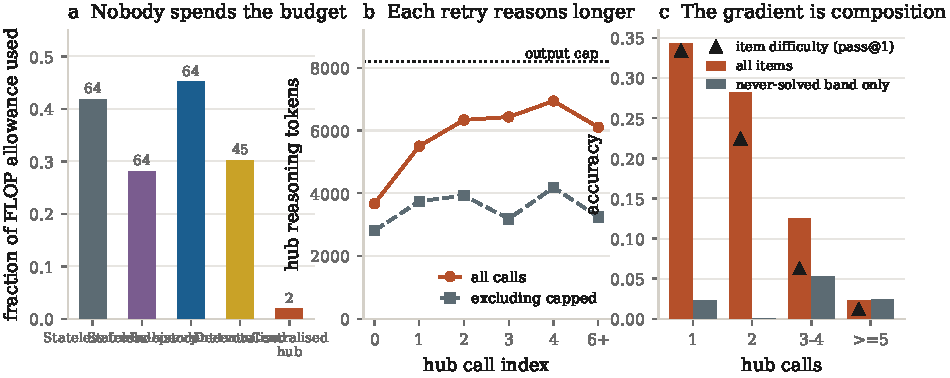
\includegraphics[width=\linewidth]{figures/f4_compute.pdf}
\caption{Realised compute and the hub's loop. \textbf{(a)} Fraction of the FLOP allowance actually spent, with mean calls above each bar; every topology stops on a structural cap. \textbf{(b)} Hub reasoning length by call index, with and without calls that hit the output cap. \textbf{(c)} Accuracy by hub call count, against item difficulty and against the same buckets inside the never-solved band.}
\label{fig:compute}\end{figure}

\subsection{\ax{C3} interaction depth: peer revision is a conformity process}\label{sec:rounds}

\trend{\ax{C3}$\times$\bx{B4} --- Rounds buy consensus and certainty; the first round buys whatever accuracy there is. \textsc{confirmed}}
Over eight rounds of peer revision (Figure~\ref{fig:rounds}), mean stated confidence rises monotonically from 0.853 to 0.930, and answer agreement rises with it, ending at 0.814 under the official grouping with \textbf{57.8\%} of episodes unanimous. Per-candidate correctness moves 0.314 to 0.320 --- essentially all of it in round 1 --- while \textbf{oracle coverage falls from 0.438 to 0.352}. The team converges on an answer, becomes more certain of it, and loses the correct answers some members were holding.

\trend{\ax{C3}$\times$\bx{B4} --- Members conform to the majority rather than to the truth. \textsc{confirmed}}
Across 14{,}039 labelled member-transitions, a member in the minority changes its answer at \textbf{0.626} against \textbf{0.041} for a member already in the plurality --- a 15-fold ratio. The changes are almost exactly a wash on correctness: \textbf{121 wrong$\to$correct against 106 correct$\to$wrong}, a net gain of 15 over fourteen thousand transitions. In the 32 episodes where exactly one member was right at the root, \textbf{75\% lost that answer} by the final round. Confidence rises after switching (0.898 before, 0.916 after) while non-switchers hold steady at 0.925.

\trend{\ax{C1}$\times$\bx{B4} --- Peer content, not the extra generation pass, is the active ingredient. \textsc{confirmed}}
The matched control settles this. One peer-informed revision round changes 39.2\% of answers; one \emph{private} revision round --- identical prompt structure, same roots, peers removed --- changes 8.5\%, and alters no vote outcome. Whatever revision does here, it is driven by reading other agents, not by thinking again.

\begin{figure}[H]\centering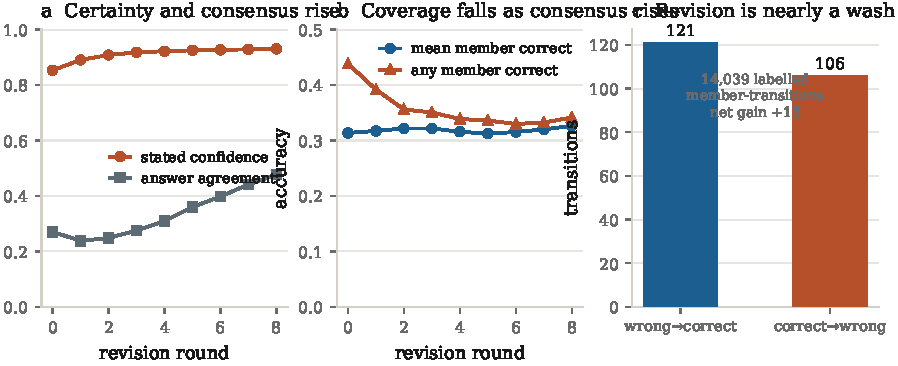
\includegraphics[width=\linewidth]{figures/f10_rounds.pdf}
\caption{Peer revision round by round. \textbf{(a)} Certainty and consensus rise together. \textbf{(b)} Mean member correctness is flat after round 1 while the chance any member is right falls. \textbf{(c)} Answer changes are almost balanced between fixing and breaking.}
\label{fig:rounds}\end{figure}

\subsection{\ax{C2} team size buys coverage that never reaches the answer}

\trend{\ax{C2}$\times$\bx{B2}/\bx{B3} --- More agents means more correct answers in the pool and not more correct answers delivered. \textsc{confirmed}}
For peer revision from $N{=}1$ to $N{=}9$ on 100 items, oracle coverage rises 0.32 to 0.45 while the voted answer rises 0.29 to 0.33; the delivered accuracy interval covers zero. For independent sampling the axis does not exist at all: all five levels are byte-identical episodes (\S\ref{sec:nominal}), fixed at 0.30 delivered and 0.52 oracle. Team size is a \emph{pool-quality} axis, and this system has no mechanism that converts pool quality into answers.

\subsection{\ax{C4} compute allowance is inert above the smallest level}\label{sec:budget}

\trend{\ax{C4}$\times$\bx{B1} --- Quadrupling the allowance is worth one to three points, because caps bind first. \textsc{confirmed}}
Paired within items, $B_4-B_1$ is $+0.02$ $[-0.02,+0.06]$ for independent sampling, $+0.03$ $[0.00,+0.07]$ for peer revision, $+0.02$ $[-0.02,+0.06]$ for the hub. At $B_1$ the budget genuinely binds --- 77\% of independent-sampling episodes stop on \textsc{budget} having spent 89\% of the allowance --- but by $B_4$ nothing stops on budget at all. The hub is the extreme case: it spends 1.9--3.8\% of its allowance at every level, so its budget contrasts are exactly zero.

\begin{tabular}{lccccccl}
\toprule
& \multicolumn{3}{c}{accuracy} & \multicolumn{3}{c}{fraction of allowance spent} & \\
\cmidrule(lr){2-4}\cmidrule(lr){5-7}
Routing topology & B1 & B2 & B4 & B1 & B2 & B4 & B4$-$B1 paired \\
\midrule
Stateless-fresh & 0.280 & 0.290 & 0.307 & 0.87 & 0.66 & 0.42 & +0.020 [-0.020, +0.060] \\
Stateless-history & 0.290 & 0.290 & 0.312 & 0.75 & 0.48 & 0.28 & +0.010 [+0.000, +0.030] \\
Independent+vote & 0.340 & 0.350 & 0.328 & 0.89 & 0.72 & 0.45 & +0.020 [-0.020, +0.060] \\
Decentralised & 0.320 & 0.340 & 0.302 & 0.72 & 0.57 & 0.30 & +0.030 [+0.000, +0.070] \\
Centralised hub & 0.260 & 0.280 & 0.287 & 0.03 & 0.04 & 0.02 & +0.020 [-0.020, +0.060] \\
\bottomrule
\end{tabular}
\vspace{-2pt}
\captionof{table}{\ax{C4}$\times$\bx{B1}, \bx{B6} on the shared 100-item budget panel. The realised spend column is the reason the accuracy column is flat.}
\label{tab:budget}

\subsection{\ax{C5} model scale}

\trend{\ax{C5}$\times$\bx{B1} --- 8B matches 32B at matched allowance; the ordering reverses by domain. \textsc{confirmed}}
On the dense panel (Figure~\ref{fig:scale}, Table~\ref{tab:scale}) 8B is within noise of 32B on two of three topologies and beats 14B, whose deficit is exam-specific ($+0.058$ $[+0.004,+0.116]$ on the exam, $+0.004$ $[-0.053,+0.062]$ on code). Across domains, code accuracy rises monotonically with scale while exam accuracy does not, and multiple-choice exam items actually peak at 4B.

\trend{\ax{C5}$\times$\bx{B7} --- The small model's deficit is substantially mechanical. \textsc{confirmed}}
4B produces unparseable structured answers far more often than its larger siblings, and on code its schema-failure rate is 0.411 against 0.006 for 8B. Its pools are thinner at comparable oracle coverage --- it is losing answers at the output contract, not only at the reasoning.

\trend{\ax{C5}$\times$\bx{B5} --- Bigger models are more confident, not better calibrated --- but the naive version of this is an artefact. \textsc{narrowed}}
Stated confidence rises with scale while accuracy barely moves. The obvious reading is wrong in one respect: 8B emits a literal 0.50 on \textbf{59\%} of candidates, 4B on 42\% and 14B on 13\%, against 0.8\% at 32B. Excluding that value, stated confidence is 0.83--0.86 at every scale. The 0.50 is not a content-free default, though: on exam items its per-item frequency correlates $-0.447$ with accuracy, so it functions as an \emph{abstention} signal. Small checkpoints really are better calibrated --- because they abstain, not because their non-abstaining confidences are better.

\begin{figure}[H]\centering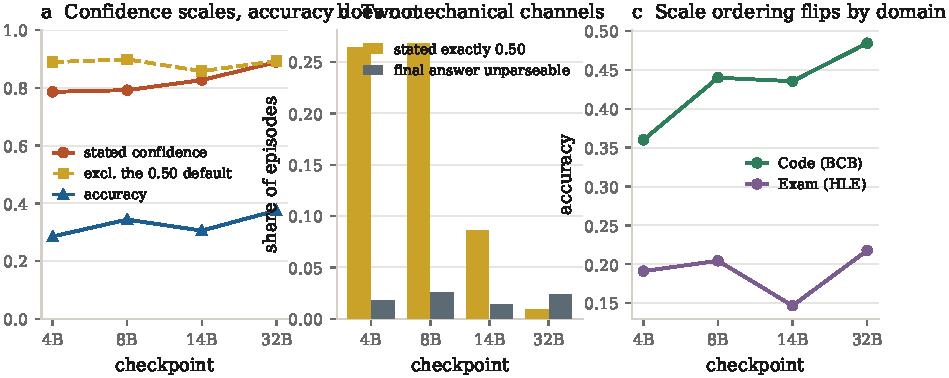
\includegraphics[width=\linewidth]{figures/f8_scale.pdf}
\caption{Model scale. \textbf{(a)} Confidence tracks scale; accuracy does not; excluding the 0.50 default removes most of the confidence trend. \textbf{(b)} Two mechanical channels: the 0.50 abstention and unparseable finals. \textbf{(c)} The scale ordering differs by domain.}
\label{fig:scale}\end{figure}

\begin{tabular}{lcccccccc}
\toprule
& \multicolumn{3}{c}{accuracy} & \multicolumn{3}{c}{stated confidence} & & \\
\cmidrule(lr){2-4}\cmidrule(lr){5-7}
Checkpoint & pooled & exam & code & all & excl.\ 0.50 & share $=$0.50 & valid final & Brier \\
\midrule
4B & 0.285 & 0.191 & 0.360 & 0.786 & 0.889 & 0.264 & 0.982 & 0.475 \\
8B & 0.344 & 0.204 & 0.440 & 0.792 & 0.899 & 0.268 & 0.975 & 0.441 \\
14B & 0.305 & 0.147 & 0.436 & 0.827 & 0.858 & 0.086 & 0.986 & 0.474 \\
32B & 0.375 & 0.218 & 0.484 & 0.889 & 0.893 & 0.010 & 0.977 & 0.490 \\
\bottomrule
\end{tabular}
\vspace{-2pt}
\captionof{table}{\ax{C5} against \bx{B1}, \bx{B5}, \bx{B7}. The 32B row is the flagship panel restricted to the dense-panel items and topologies.}
\label{tab:scale}

\subsection{\ax{C7} aggregation: the bottleneck}\label{sec:selection}

\trend{\ax{C7}$\times$\bx{B3} --- Every selector reads a signal that is not correctness. \textsc{confirmed}}
Independent sampling puts a correct answer in the pool on \textbf{54.3\%} of items and delivers \textbf{32.8\%} --- a 21.5-point selection gap (Table~\ref{tab:selection}, Figure~\ref{fig:selection}). Plurality voting beats drawing a random valid candidate by only $+0.026$ $[+0.004,+0.047]$, and the pointwise LLM judge --- the same checkpoint, scoring each candidate --- beats it by $+0.006$ $[-0.020,+0.031]$, i.e.\ not at all. On the exam the judge's pairwise discrimination is \emph{below} chance (AUC 0.454 $[0.436,0.471]$): it prefers the wrong candidate slightly more often than not, while systematically picking higher-confidence ones (0.900 against the vote's 0.855).

\trend{\ax{C7}$\times$\ax{C9} --- Voting fails for opposite reasons in the two domains. \textsc{confirmed}}
On code, 144 of 200 pools have a winning class holding $\le$10\% of the pool and 20\% are entirely singletons, so the ``vote'' is decided by a deterministic tie-break; \textbf{77\%} of covered-but-wrong code pools fail structurally (all-singleton, or equivalent correct programs split across syntactic classes), and the vote picks wrong 6--8\% of the time even when correct programs are the majority. On the exam the vote has real signal but fails confidently: \textbf{91\%} of covered-but-wrong exam pools are a correct minority buried under a wrong consensus, with a median correct class of 2 candidates against a winning class of 27.

\trend{\ax{C4}$\times$\bx{B3} --- Test-time compute widens the gap it is supposed to close. \textsc{confirmed}}
pass@$k$ climbs steadily with samples (exam 0.127$\to$0.295, code 0.412$\to$0.600 from $k{=}1$ to 10) while vote@$k$ and judge@$k$ are flat (pooled 0.281$\to$0.294 and 0.281$\to$0.296). The pooled gap between what the pool contains and what the selector extracts grows from $-0.011$ at $k{=}1$ to $+0.153$ at $k{=}10$ (Figure~\ref{fig:ttc}). Sampling is the axis that works; harvesting is the axis that does not.

\begin{figure}[H]\centering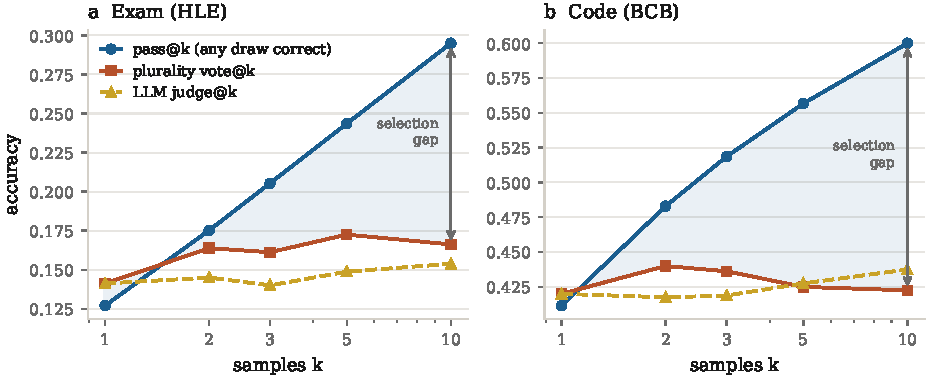
\includegraphics[width=\linewidth]{figures/f5_ttc.pdf}
\caption{Test-time compute widens the generation--verification gap. Shaded: the pool's correct answers that no selector retrieves.}
\label{fig:ttc}\end{figure}

\begin{figure}[H]\centering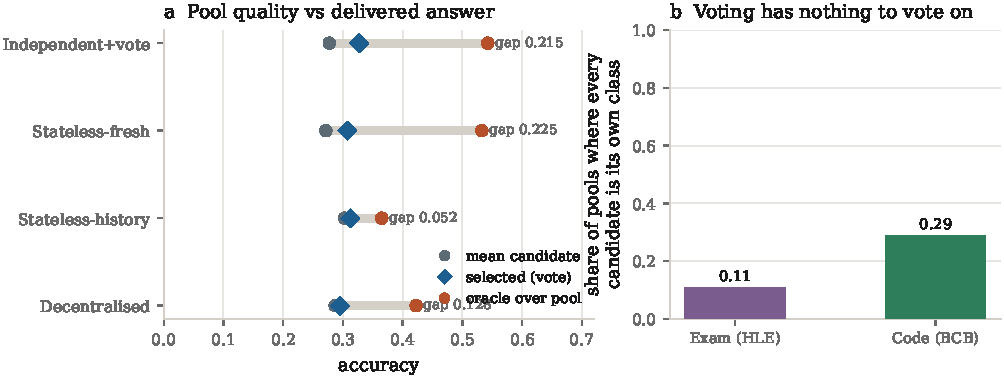
\includegraphics[width=\linewidth]{figures/f6_selection.pdf}
\caption{\textbf{(a)} Mean candidate, delivered answer and oracle over the same sealed pool. \textbf{(b)} On code, syntactic grouping leaves the vote with nothing to count.}
\label{fig:selection}\end{figure}

\begin{tabular}{lcccccc}
\toprule
Routing topology & mean candidate & vote & LLM judge & oracle & gap & all-singleton \\
\midrule
Independent+vote & 0.277 & 0.328 & 0.307 & 0.542 & 0.215 & 0.200 \\
Stateless-fresh & 0.271 & 0.307 & 0.305 & 0.532 & 0.225 & 0.190 \\
Stateless-history & 0.303 & 0.312 & 0.307 & 0.365 & 0.052 & 0.010 \\
Decentralised & 0.287 & 0.295 & 0.292 & 0.422 & 0.128 & 0.010 \\
\bottomrule
\end{tabular}
\vspace{-2pt}
\captionof{table}{\ax{C7}$\times$\bx{B3} on module-A archive pools, 400 items.}
\label{tab:selection}

\subsection{\ax{C1}, \ax{C6} \texorpdfstring{$\times$}{x} \bx{B5}: information sharing inflates certainty}

\trend{\ax{C1}$\times$\bx{B5} --- The more an agent sees of other agents, the more certain and worse calibrated it is. \textsc{confirmed}}
Ordered by Brier (Table~\ref{tab:calibration}, Figure~\ref{fig:calibration}): independent+vote 0.476, stateless-fresh 0.527, the hub 0.537, peer revision 0.576, stateless-with-history 0.579. The share of answers stated at $\ge$0.95 confidence runs from 0.191 for independent sampling to 0.766 for the history-carrying policy. Accuracy over that range moves by about two points; stated certainty moves by 58.

\trend{\bx{B5} --- Confidence is ordinal between items and empty within them. \textsc{confirmed}}
The reliability curve is monotone --- $\le$0.5 confidence yields 12\% accuracy, $\ge$0.95 yields 43\% --- while sitting 45--62 points above the diagonal. But between siblings on the same question, confidence carries essentially nothing: within-item AUC is 0.495 pooled over thousands of candidate pairs, and pooled within-item resolution is $+0.0004$ $[-0.0043,+0.0050]$. Confidence encodes \emph{how hard the question is}, which is why it looks informative in aggregate and is useless for choosing an answer.

\trend{\bx{B5} --- The system's explicit self-forecast is a copy of the confidence it just read. \textsc{confirmed}}
Asked to estimate the probability that the team's selected answer is correct, the reader reproduces the selected candidate's own stated confidence verbatim in \textbf{896 of 896} parsed forecasts for the personal channel, and 66--98\% of the time for the team channel. Every stated-probability channel scores Brier 0.44--0.59 against 0.22 for a constant base rate. Post-hoc recalibration, by contrast, is worth an enormous amount: a dev-fitted logistic map cuts Brier from 0.491 to 0.216.

\trend{\ax{C6}$\times$\bx{B5} --- Telling agents they will be voted on lowers their stated confidence without changing what they write. \textsc{unverified}}
Across the 400-item framing banks, no framing contrast moves accuracy: $11-00$ is $+0.007$ $[-0.007,+0.021]$ at pass@1 and $-0.023$ $[-0.053,+0.005]$ at pass@10. But the vote-aware framing lowers stated confidence by $-0.036$ $[-0.053,-0.017]$. The same comparison shows an accuracy gain of $+0.063$ $[+0.011,+0.126]$, which we do \textbf{not} believe: the 10-draw banks on the same items show no such effect, and it does not replicate at 8B. It is most likely a seed/aliasing artefact of comparing two module arms, and is flagged here rather than reported as a trend.

\begin{figure}[H]\centering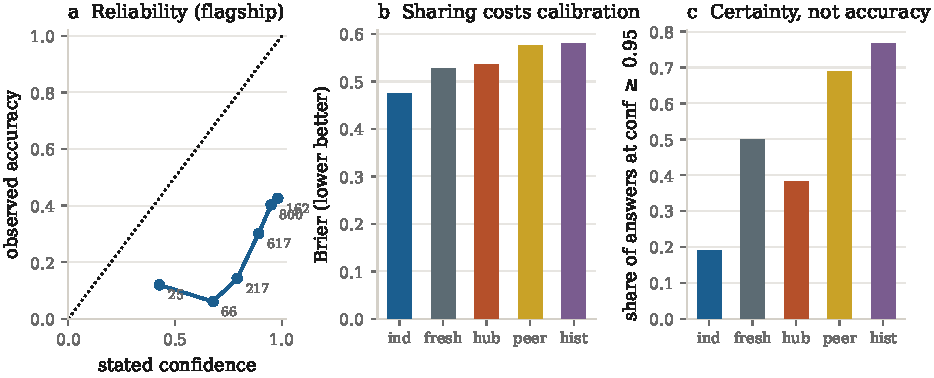
\includegraphics[width=\linewidth]{figures/f7_calibration.pdf}
\caption{\textbf{(a)} Reliability on the flagship panel: monotone, and far above the diagonal. \textbf{(b)} Brier by topology, ordered by how much peer information each agent sees. \textbf{(c)} The same ordering in the share of near-certain answers.}
\label{fig:calibration}\end{figure}

\begin{tabular}{lcccccc}
\toprule
Routing topology & accuracy & stated conf. & bias & Brier & share $\ge$0.95 & resolution \\
\midrule
Independent+vote & 0.343 & 0.855 & 0.512 & 0.476 & 0.191 & 0.045 \\
Stateless-fresh & 0.321 & 0.890 & 0.568 & 0.527 & 0.499 & 0.055 \\
Centralised hub & 0.307 & 0.883 & 0.575 & 0.537 & 0.382 & 0.041 \\
Decentralised & 0.325 & 0.931 & 0.605 & 0.576 & 0.688 & 0.031 \\
Stateless-history & 0.332 & 0.937 & 0.604 & 0.579 & 0.766 & 0.024 \\
\bottomrule
\end{tabular}
\vspace{-2pt}
\captionof{table}{\ax{C1}$\times$\bx{B5} on the flagship panel, restricted to episodes that stated a confidence (so accuracies differ slightly from Table~\ref{tab:policies}, which scores missing finals as wrong). Resolution is mean confidence given correct minus given wrong.}
\label{tab:calibration}

\subsection{Documented nulls}\label{sec:nulls}

These axes were varied and did not move the outcome. Each is a design decision someone would otherwise spend effort on.

\begin{itemize}
\item \ax{C6}\textbf{ prompt framing on correctness.} All four $2\times2$ cells sit within 0.011 of each other at pass@1 (0.269, 0.272, 0.266, 0.276) and every paired interval covers zero at every $k$. The one directional signal is that the both-framings cell has the \emph{lowest} pass@10 (0.425 against 0.448).
\item \ax{C2}\textbf{ team size for independent sampling.} Not an axis: identical episodes at every level.
\item \ax{C2}\textbf{ team size for the hub.} 0.28, 0.27, 0.24, 0.28, 0.28 across $N=1..9$, with calls fixed at 2.2--2.5. The hub does not use its roster.
\item \ax{C3}\textbf{ consumer degree.} Focal accuracy 0.174, 0.217, 0.217, 0.200, 0.239 across degree $0,1,2,4,8$ on 46 exam items --- weakly positive, entirely inside noise, and the module lost its whole code half so no pooled estimate exists.
\item \ax{C4}\textbf{ budget above the smallest level} (\S\ref{sec:budget}).
\item \ax{C7}\textbf{ the LLM judge over the vote.} Never better, worse on the exam.
\item \textbf{Confidence-aware selectors.} Max-confidence, confidence-weighted voting and top-quartile plurality all land within 1.5 points of plain plurality; every interval against a random valid draw covers zero.
\item \ax{C8}\textbf{ repetition} does separate the topologies on \bx{B8} --- the hub is the least stable (accuracy range 0.133 across repeats, within-item SD 0.162) and peer revision the most stable (0.033, 0.055) --- but stability tracks nothing else, and on the exam it is floor-induced.
\end{itemize}

\section{Configuration \texorpdfstring{$\to$}{->} mechanism}\label{sec:cm}

\subsection{\ax{C1} \texorpdfstring{$\times$}{x} \mx{M1}--\mx{M4}: what peer exposure does to the answer state}

\trend{\ax{C1}$\times$\mx{M1} --- Peer-exposed agents commit their answers from a lower-dimensional state. \textsc{confirmed}}
At the token closing the answer object, block 31, paired on 109 items: participation ratio \textbf{2.362 for independent solvers against 1.840} for peer-exposed members, entropy effective rank 2.815 against 2.177 (Table~\ref{tab:geometry}). It holds within domain (code 2.38$\to$1.71; exam 2.37$\to$1.99) and at all three depths, and it reproduces to five decimal places when recomputed from the raw 5{,}120-dimensional vectors rather than the shipped table.

\trend{\ax{C1}$\times$\mx{M2} --- It is anisotropy, not convergence. \textsc{narrowed}}
This is the correction that matters most in the document. The mean distance between the five agents' answer states is \textbf{unchanged} --- 52.46 for independent solvers, 52.50 for peer-exposed members, a ratio of 1.001. Total variance is if anything \emph{higher} for the peer-exposed arm (1{,}660 against 1{,}887, ratio 1.14) and so is angular dispersion (ratio 1.17). What changes is the shape: the share of variance on the leading eigenvector rises from \textbf{0.612 to 0.740}, the nearest pair closes by 29\% and the farthest pair opens by 9\%. Peer exchange concentrates the ensemble's variation onto a single dominant axis without shrinking it --- a tight cluster with one member strung out --- and the participation ratio registers that reshaping as if it were contraction. Reading only the scale-free family produced, in this study, a published claim that the agents' representations ``converge''. They do not.

\trend{\ax{C1}$\times$\mx{M5} --- The effect is specific to the committed answer, not the reasoning. \textsc{confirmed}}
Along the trajectory (Figure~\ref{fig:geometry}a), the two arms are statistically indistinguishable through the middle of generation --- participation ratio 2.56 against 2.52 at 32 tokens ($p=0.56$) and 3.60 against 3.61 at 128 ($p=0.75$) --- diverge slightly by 512 tokens, and separate sharply only at the answer token. At the prompt the arms differ in the opposite direction, but that comparison is close to definitional: independent solvers share one byte-identical prompt, and both arms' prompt states are two orders of magnitude closer together (mean pairwise 1.02 and 8.11) than they are at the answer token (52). \emph{Orchestration does not change the geometry of the reasoning trajectory; it changes the geometry of the commitment.}

\begin{figure}[H]\centering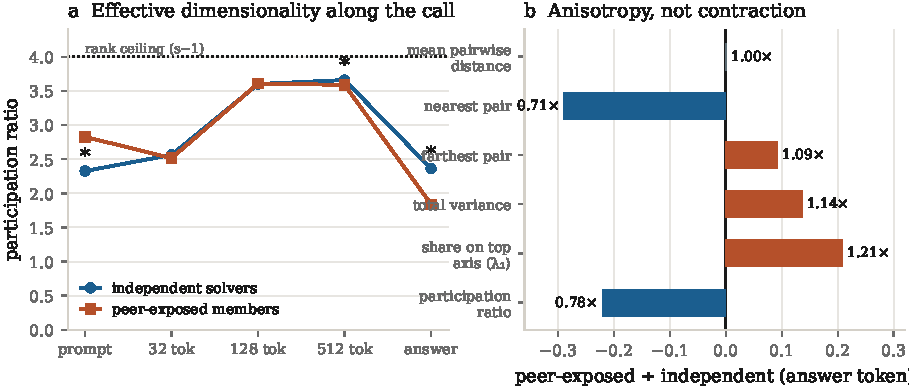
\includegraphics[width=\linewidth]{figures/f11_geometry.pdf}
\caption{\textbf{(a)} Effective dimensionality of the five comparable agent states along one call. The arms coincide through generation and separate at the answer token ($\ast$: $p<0.01$). \textbf{(b)} At that anchor, decomposed: the mean separation is unchanged and the total variance slightly larger, while the share on the leading axis rises --- anisotropy, not contraction.}
\label{fig:geometry}\end{figure}

\begin{tabular}{llcccc}
\toprule
Observable & family & independent & peer-exposed & ratio & $p$ \\
\midrule
participation ratio & scale-free & 2.362 & 1.840 & 0.779 & $<$1e-16 \\
entropy effective rank & scale-free & 2.815 & 2.177 & 0.773 & $<$1e-16 \\
share of variance on $\lambda_1$ & scale-free & 0.612 & 0.739 & 1.209 & $<$1e-16 \\
total variance & scale-carrying & 1660.1 & 1886.8 & 1.137 & 0.027 \\
mean pairwise distance & scale-carrying & 52.458 & 52.500 & 1.001 & 0.98 \\
nearest pair & scale-carrying & 29.455 & 20.923 & 0.710 & $<$1e-16 \\
farthest pair & scale-carrying & 73.093 & 79.847 & 1.092 & 0.016 \\
mean pairwise cosine distance & angular & 0.051 & 0.060 & 1.170 & 0.0074 \\
mean state norm & scale-carrying & 180.4 & 178.2 & 0.988 & $<$1e-16 \\
\bottomrule
\end{tabular}
\vspace{-2pt}
\captionof{table}{\ax{C1}$\times$\mx{M1}--\mx{M4} at the answer anchor, block 31, 109 paired items. Recomputed from raw \texttt{fp16} vectors.}
\label{tab:geometry}

\begin{aside}{What confounds this contrast, and what does not}
\textbf{Not prompt-matched.} Peer-exposed members run a truthful native framing while the independent arm draws from vote-aware framing on 84 of 109 items and neutral framing on the other 25. Both framings give the same sign, so framing is not the driver.
\textbf{Not length-matched.} At the answer anchor a peer-exposed member's context is 2{,}153 prompt tokens against 379, and it writes shorter answers (1{,}694 completion tokens against 3{,}242). Completion length \emph{does} affect this geometry: within independent solvers alone, the five longest completions give a lower participation ratio than the five shortest (exam 2.38 against 2.79, $p=0.007$). Crucially this runs \textbf{against} the observed effect --- peer-exposed members write shorter answers, which predicts \emph{higher} dimensionality, and we observe lower. Length cannot explain the result, though context length remains unseparated from topology.
\textbf{No within-episode baseline.} Only one root member per peer-revision episode was captured, so ``before and after peer exposure'' is a between-arm contrast everywhere in this data, never a within-episode one. This is the single most valuable missing measurement.
\end{aside}

\subsection{\ax{C1} \texorpdfstring{$\times$}{x} \mx{M9}: the harness is written all over the reader's state}

\trend{\ax{C1}$\times$\mx{M7} --- A linear probe identifies the orchestration architecture almost perfectly, from the representation of its handoff report. \textsc{confirmed}}
The same reader model reads a compiled report from each of the three topologies on each item. From its state at the end of the report, a 3-way probe recovers which topology produced it with accuracy \textbf{0.989} at block 31 (0.975 at block 15, 0.998 at block 47) against a chance rate of 0.333. From the task span alone --- before any evidence has been read --- it recovers \textbf{0.342}, i.e.\ nothing. The architectural signature is entirely in the evidence, and it is close to linearly separable.

\trend{\ax{C1}$\times$\mx{M9} --- How far the evidence moves the reader tracks pool quality, not answer quality. \textsc{unverified}}
The compiled report displaces the reader's state by 0.79--0.82 of the task-state norm, similarly for all three topologies. That displacement correlates $+0.099$ ($p=0.038$, code) with whether the pool contained a correct answer and $+0.005$ ($p=0.91$) with whether the delivered answer was right --- the coverage/selection split of \S\ref{sec:selection}, reappearing inside the model.

\section{Mechanism \texorpdfstring{$\to$}{->} behaviour}\label{sec:mb}

\subsection{\mx{M7}: what the state knows, and when}

\trend{\mx{M7}$\times$\bx{B1} --- Difficulty is legible before generation starts; correctness is barely legible after it ends. \textsc{confirmed}}
From the prompt state alone, averaged over an item's draws, a ridge probe predicts that item's eventual pass rate at $\rho=0.29$ (Figure~\ref{fig:probes}a, Table~\ref{tab:probes}). By contrast, a probe asked which \emph{sibling} candidate on the same question is correct reaches only 0.54--0.63 AUC on the exam and 0.47--0.53 on code. Pooled AUC looks respectable at 0.63--0.70 across blocks, but pooling mixes easy and hard items --- it is largely re-reading difficulty.

\trend{\mx{M7}$\times$\bx{B4} --- Mainstream-ness is more legible than correctness. \textsc{confirmed}}
Asked instead whether a candidate will join the plurality, the same within-item probe reaches 0.566 on the exam and \textbf{0.590} on code --- higher than the correctness probe in both domains, and on code where correctness is at chance this is the only within-item signal that exists. The residual stream at the answer token carries more information about whether an answer is typical than about whether it is right.

\trend{\mx{M7}$\times$\bx{B5} --- The confidence value is not represented before it is written. \textsc{confirmed}}
A ridge probe recovers the stated confidence with grouped-CV $R^2=0.097$ at 128 generated tokens and $0.121$ at 512, with within-item $\rho$ of 0.012 and 0.029 --- nothing. At the answer token $R^2$ jumps to \textbf{0.627}. The number appears to be produced at commitment time rather than tracked during reasoning, which is consistent with its behavioural profile: ordinal across items (difficulty is available early) and empty within them.

\begin{figure}[H]\centering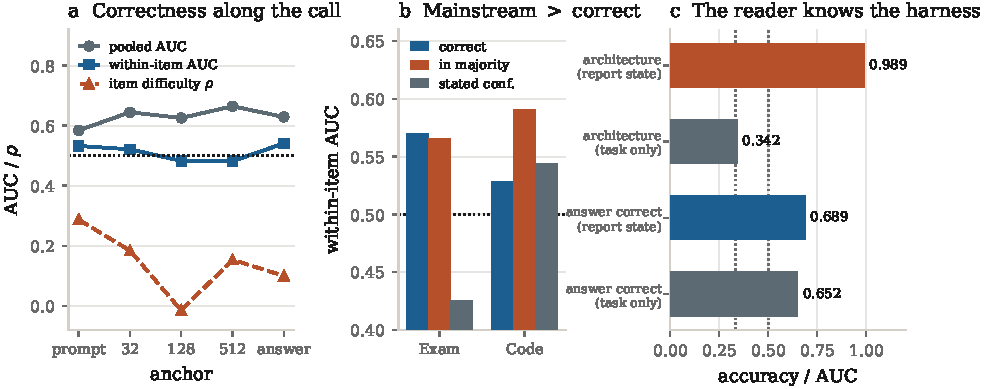
\includegraphics[width=\linewidth]{figures/f13_probes.pdf}
\caption{\textbf{(a)} Correctness probes along the call: the pooled curve tracks difficulty, the within-item curve stays near chance. \textbf{(b)} Within an item, majority membership is more decodable than correctness, and stated confidence is at chance. \textbf{(c)} The reader's state identifies the harness almost perfectly and the answer's correctness barely better than the task text alone.}
\label{fig:probes}\end{figure}

\begin{tabular}{llcl}
\toprule
Decoded target & site & value & metric \\
\midrule
which orchestration produced this report & report state, b31 & 0.989 & 3-way acc., chance 0.333 \\
\quad from the task text alone & task anchor, b31 & 0.342 & 3-way acc. \\
item difficulty & prompt, b31 & 0.287 & Spearman $\rho$, item level \\
whether the delivered answer is right & report state, b31 & 0.689 & AUC \\
\quad from the task text alone & task anchor, b31 & 0.652 & AUC \\
is \emph{this} candidate right (exam) & answer token, b31 & 0.570 & within-item AUC \\
is \emph{this} candidate right (code) & answer token, b31 & 0.529 & within-item AUC \\
will it join the majority (exam) & answer token, b31 & 0.566 & within-item AUC \\
will it join the majority (code) & answer token, b31 & 0.590 & within-item AUC \\
the stated confidence value & 128 tokens in & 0.097 & grouped-CV $R^2$ \\
the stated confidence value & 512 tokens in & 0.121 & grouped-CV $R^2$ \\
the stated confidence value & answer token & 0.627 & grouped-CV $R^2$ \\
hub will make extra calls (exam) & hub prompt, b31 & 0.603 & AUC \\
\quad within the never-solved band & hub prompt, b31 & 0.593 & AUC, difficulty held \\
\bottomrule
\end{tabular}
\vspace{-2pt}
\captionof{table}{\mx{M7} decodability. ``Within-item'' removes the item mean, so only variation between siblings on one question counts.}
\label{tab:probes}

\subsection{\mx{M1}--\mx{M3} \texorpdfstring{$\times$}{x} \bx{B4}: geometry and consensus}

\trend{\mx{M1}$\times$\bx{B4} --- Episodes that reach unanimity are more one-dimensional but \emph{more} spread out. \textsc{narrowed}}
On the exam, unanimous peer-revision episodes have participation ratio 1.805 against 2.437 for split ones (Welch $p=0.013$; agreement correlates $\rho=-0.28$), and this is not difficulty: the partial correlation given item pass rate is $-0.280$, essentially unchanged. But on every scale-carrying metric the sign reverses --- unanimous episodes have mean pairwise distance \textbf{52.3 against 41.4} ($p=0.020$), farthest pair 79.8 against 59.4, angular dispersion 0.058 against 0.039, all correlating \emph{positively} with agreement. Token-level consensus coincides with a more strung-out, lower-rank state geometry, not with members being drawn together. The effect is also thin: it rests on about a dozen items, and dropping the three most dispersed split episodes takes $p$ to 0.076.

\trend{\mx{M3}$\times$\bx{B4} --- On code the consensus signal is in the norm, and it is the strongest association in the study. \textsc{confirmed}}
The participation ratio shows nothing on code (1.850 unanimous against 1.842 split, $p=0.96$), which invited the conclusion that the domain was empty. It is not: mean state norm correlates $\rho=+0.389$ ($p<10^{-4}$) with agreement there --- the single strongest mechanism--behaviour association anywhere in this data, and the only one that would survive a correction across all sixteen metric-by-domain tests. Which metric family you read determines which domain looks empty.

\trend{\mx{M1}--\mx{M4}$\times$\bx{B1} --- None of it predicts correctness. \textsc{confirmed}}
In no cell does any geometric observable separate episodes that end right from episodes that end wrong: participation ratio 2.19 against 1.92 on the exam ($p=0.33$), 1.84 against 1.85 on code ($p=0.99$), and every other metric likewise. The geometry tracks consensus and difficulty; it does not track truth.

\trend{\mx{M1}$\times$\bx{B2} --- On code, a high-dimensional sampling distribution marks items the model does not have. \textsc{unverified}}
Using all $\approx58$ available draws instead of a fixed five, an item's whole answer-state distribution has participation ratio 4.79 on average. On code, candidate accuracy falls across terciles of that dimensionality from \textbf{0.548 to 0.371}; on the exam it is flat (0.157, 0.130, 0.143) and at floor. Spread in answer states is not diversity to be harvested --- where a reliable grader exists, it marks failure.

\section{Mediation and colinearity}\label{sec:med}

The atlas would be far more useful if it could say that a configuration changes behaviour \emph{through} a mechanism. It cannot, and the reasons are worth stating precisely, because they are the design brief for the next run.

\paragraph{What mediation would require here.} For \ax{C1}$\to$\mx{M}$\to$\bx{B} we would need (i) the configuration to move the mechanism, (ii) the mechanism to move the behaviour with the configuration held fixed, and (iii) the configuration's effect on behaviour to shrink when the mechanism is conditioned on. This study establishes (i) robustly for the answer-state geometry, gets (ii) only for consensus --- never for correctness --- and cannot attempt (iii) at all.

\paragraph{Why (iii) is unavailable.} Three structural features block it.
\begin{itemize}
\item \textbf{No within-episode baseline.} Only one root member per peer-revision episode was captured, so every mechanistic comparison is between arms rather than before/after inside one episode. Any item-level or episode-level confounder is fully aliased with the topology.
\item \textbf{The arms differ in more than topology.} Framing differs (native-truthful against vote-aware on 84 of 109 items), and context length differs by a factor of 5.7 at the anchor. We can show the length confound runs against the effect --- shorter completions give \emph{higher} dimensionality, and the peer-exposed arm writes shorter answers --- but we cannot separate ``carrying peer packets in context'' from ``being in a peer-revision protocol'', because they are the same intervention.
\item \textbf{The mechanism does not move the behaviour we care about.} Every geometric observable is null against correctness in every cell. A mediator of an accuracy effect must correlate with accuracy; none does. The one strong mechanism--behaviour link, norm against agreement on code ($\rho=+0.389$), mediates a \emph{consensus} outcome, and consensus is itself not predictive of correctness at $N\ge5$.
\end{itemize}

\paragraph{Colinearity, stated plainly.} The dominant confounder throughout the atlas is \ax{C10}, item difficulty. It is decodable from the prompt state before generation ($\rho=0.29$), it determines whether the hub enters a retry loop (multi-call rate 0.38 on never-solved items against 0.16 elsewhere), it drives the pooled correlation between state norm and accuracy (which vanishes within domain), and it generates the pooled-versus-conditional illusion of \S\ref{sec:difficulty}. \textbf{Any configuration--behaviour or mechanism--behaviour association in this document that has not been split by domain and by difficulty band should be assumed to be partly difficulty.} Where we have done that split, we report it.

\paragraph{The one thing that does look like a mechanism with a behavioural consequence.} Peer exposure concentrates the answer state onto one axis (\S\ref{sec:cm}); peer exposure raises agreement and stated confidence without raising accuracy (\S\ref{sec:rounds}); and on the exam the degree of concentration tracks the degree of agreement, with difficulty partialled out. That is a coherent story --- consensus is visible in the representation before it is visible in the vote --- and it is exactly the story the current design cannot distinguish from ``longer contexts produce more anisotropic states''. The instrument that separates them is in \S\ref{sec:followups}, item 1.

\part{Positioning and direction}\label{part:pos}

\section{Related work and novelty}\label{sec:novelty}

We put 34 claims to a literature search, each assessed by one agent and then attacked by an independent adjudicator instructed to demote over-generous calls; \textbf{11 verdicts were changed}. The result is a sharp corrective to how novel a large study feels from the inside: \textbf{16 claims replicate} known results, \textbf{16 extend} them into a new regime, \textbf{2 contradict} prior work, and \textbf{none survives as novel}. Both claims we initially believed were new --- the anchor-specificity of the orchestration effect and the dispersion-by-dimensionality signature of consensus --- were demoted on the second pass, each by a precedent the first assessor had missed.

\begin{aside}{How to read the verdicts}
Citations were gathered by automated literature search and are reported as the assessors found them; we spot-verified the load-bearing 2026 references directly and corrected two characterisations (below). ``Replication'' is not a criticism --- most of these results were previously shown on different models, single axes, or uncontrolled comparisons, and the contribution here is that they hold together in \emph{one} factorial design on one model family with shared items. ``Extension'' is where most of this study's value sits: a known phenomenon measured on a new substrate, crossed with a new axis, or decomposed in a way that changes what it means.
\end{aside}

\begin{longtable}{@{}p{0.9cm}p{8.8cm}p{1.9cm}p{3.2cm}@{}}
\toprule
Axis & Claim & Verdict & Closest prior work \\
\midrule
\endfirsthead
\toprule
Axis & Claim & Verdict & Closest prior work \\
\midrule
\endhead
\mx{M5} & The effect is anchor-specific: absent mid-generation, present only at the committed answer. & \vnov & \citep{wang2026truth,liang2026divergence,sun2026toolcall} \\
\mx{M2} & Unanimous episodes have \emph{more} dispersed member states arranged along fewer directions. & \vnov & \citep{ontalvilla2026agreement,li2025dispersion,zhang2026decomposing} \\
\ax{C1} & Private revision without peers is a no-op; peer content is the active ingredient. & \vcon & \citep{bertalanic2026consensus,hao2026flips,huang2024selfcorrect} \\
\ax{C7} & Confidence-aware selectors land within 1.5 points of plain plurality. & \vcon & \citep{taubenfeld2025confidence,fu2025deepconf,kang2025selfcertainty} \\
\ax{C1} & The orchestrator rarely delegates; multi-call episodes are output-cap retry loops. & \vext & \citep{cemri2025mast,gao2026decisionbench,choi2025debate} \\
\ax{C4} & 59 nominal cells collapse to 40 distinct outcome vectors under content-addressed reuse. & \vext & \citep{kapoor2024agents,shetty2025gso,tran2026single} \\
\ax{C7} & On code, syntactic grouping makes voting structurally unavailable in 77\% of failures. & \vext & \citep{jiang2026semantic,cho2026symbolic,launer2026majority} \\
\ax{C7} & On the exam, 91\% of covered-but-wrong pools are a correct minority under a wrong consensus. & \vext & \citep{cai2026arbiter,bahuguna2026backfires,phan2025hle} \\
\bx{B5} & The explicit self-forecast copies the read confidence verbatim in 896/896 cases. & \vext & \citep{shi2026confidence,spiess2025calibration,paleka2025pitfalls} \\
\ax{C5} & 8B matches 32B at matched FLOPs; the scale ordering reverses by domain. & \vext & \citep{brown2024monkeys,snell2024scaling,wunderlich2026pareto} \\
\ax{C5} & Stated confidence rises with scale while accuracy does not. & \vext & \citep{tao2025revisiting,xiong2024can,phan2025humanity} \\
\ax{C5} & Small checkpoints emit a literal 0.50 that functions as abstention, not a default. & \vext & \citep{dai2026rescaling,shen2026provable,ferdous2026small} \\
\mx{M1} & Peer-exposed agents commit from a lower-rank answer state (PR 2.36$\to$1.84). & \vext & \citep{patel2026collapse,chen2026diversity,wan2026deliberative} \\
\mx{M2} & That drop is anisotropy: mean separation unchanged, variance share on $\lambda_1$ 0.61$\to$0.74. & \vext & \citep{zhang2026simulated,steck2024cosine,rudman2022isoscore} \\
\mx{M3} & On code the consensus signal is in the norm ($\rho=+0.389$), invisible to the scale-free metric. & \vext & \citep{parupudi2026anisotropy,ontalvilla2026agreement,steck2024cosine} \\
\mx{M7} & A reader's state identifies the harness at 0.989 and answer correctness at 0.694 (0.649 from task alone). & \vext & \citep{sun2026toolcall,leong2026recognition,liu2026reader} \\
\ax{C10} & Bimodal item difficulty gates every axis; pooled averages understate conditional effects $\sim4\times$. & \vext & \citep{chen2024more,yang2025revisiting,haupt2026welfare} \\
\ax{C1} & Independent+vote beats the centralised hub at matched compute; peer revision beats neither. & \vrep & \citep{choi2025debate,smit2023mad,li2024agents} \\
\ax{C3} & Peer revision raises agreement and confidence monotonically while pool coverage falls. & \vrep & \citep{bertalanic2026consensus,zhu2026demystifying,hao2026flips} \\
\ax{C2} & A lone correct member is overturned 75--86\% of the time at $N\ge5$. & \vrep & \citep{hussain2026frontier,weng2025conformity,zhu2025conformity} \\
\ax{C3} & Round 1 delivers the whole correctness gain; rounds 2--8 cost $4.3\times$ and buy agreement. & \vrep & \citep{choi2025debate,smit2023mad,liu2024groupdebate} \\
\ax{C2} & Team size buys pool coverage ($+0.13$) but not delivered accuracy ($+0.04$). & \vrep & \citep{brown2024monkeys,li2024agents,bertalanic2026consensus} \\
\ax{C4} & pass@$k$ climbs while vote@$k$ and judge@$k$ stay flat. & \vrep & \citep{brown2024monkeys,stroebl2024flaws,chen2024calls} \\
\ax{C4} & Nominal budget is inert once call/round caps bind; 17--45\% of the allowance is spent. & \vrep & \citep{shetty2025gso,tran2026single,muennighoff2025s1} \\
\ax{C3} & Sequential compute is dominated by parallel compute at equal FLOPs. & \vrep & \citep{huang2024selfcorrect,wen2025parathinker,bertalanic2026consensus} \\
\bx{B3} & Oracle coverage 0.542 against 0.328 delivered: a 21-point selection gap. & \vrep & \citep{brown2024monkeys,qi2025parallel,stroebl2024inference} \\
\ax{C7} & Plurality adds $+0.026$ over a random valid draw; a pointwise judge adds nothing. & \vrep & \citep{liu2026jury,zhang2026judge,landesberg2026judge} \\
\bx{B5} & Confidence is ordinal between items and empty within them (within-item AUC $\approx$0.50). & \vrep & \citep{taubenfeld2025confidence,bertalanic2026consensus,xiong2024canllms} \\
\ax{C1} & Information sharing inflates certainty without improving it (Brier 0.478$\to$0.583). & \vrep & \citep{bertalanic2026consensus,nechepurenko2026coordination,prasad2025debate} \\
\bx{B5} & Post-hoc recalibration cuts Brier 0.491$\to$0.216, dwarfing every other calibration effect. & \vrep & \citep{spiess2025calibration,shen2024thermometer,campos2025multicalibration} \\
\ax{C5} & The 4B deficit is substantially a format-compliance failure (0.67 valid). & \vrep & \citep{barzelay2026varex,neveditsin2025structured,tam2024format} \\
\mx{M7} & Item difficulty is decodable from the prompt state before any token is generated. & \vrep & \citep{lugoloobi2026encode,dicicco2026code,zhu2025already} \\
\mx{M7} & Within an item, majority membership is more decodable than correctness. & \vrep & \citep{wang2026decodability,ashuach2026masked,zhang2025reasoning} \\
\mx{M7} & The stated confidence value is not represented mid-generation ($R^2$ 0.10) but is at the answer token (0.63). & \vrep & \citep{kumaran2026verbal,podolak2025read,miao2026confidence} \\
\bottomrule
\end{longtable}
\vspace{-4pt}
\captionof{table}{Novelty assessment of 34 claims. Verdicts after adversarial adjudication.}
\label{tab:novelty}

\paragraph{What was demoted, and what survives as new.} Two mechanistic claims were assessed as novel on the first pass and overturned on the second, in both cases by prior work the first assessor had not retrieved.
(i) \emph{Orchestration reshapes the commitment, not the reasoning trajectory.} \citet{turpin2023unfaithful} already establish the behavioural form of this: an influence cue moves the model's committed answer while the reasoning it produces carries no trace of the influence. Combined with the known position-dependence of hidden-state content \citep{wang2026truth}, the phenomenon is established; what is new here is the residual-stream measurement and the crossing of an orchestration manipulation with generation-position anchors.
(ii) \emph{Consensus geometry.} INSIDE \citep{chen2024inside} establishes the ``fewer directions'' half on the same substrate (hidden states, last answer token, mid layer) and the same construct (agreement among generations of one item), stating that agreeing generations leave most eigenvalues near zero. What survives is only the \emph{dissociation} --- dispersion up while dimensionality goes down --- which INSIDE conflates in a single log-determinant and \citet{ontalvilla2026agreement} reads in the opposite direction.
The pattern in both demotions is the same, and it is the lesson of \S\ref{sec:mech}: the phenomenon was known; the contribution is separating two metric families that prior work had summarised into one number.

\paragraph{The two contradictions, stated carefully.} On \ax{C7}, confidence-weighted selection, our result matches prior magnitudes almost exactly (0.4--1.6 points in \citet{taubenfeld2025confidence}, $\le$1.5 here); it is labelled a contradiction only against the broader claim that confidence-aware aggregation is a reliable improvement, which at this scale it is not. On \ax{C1}, private revision, \citet{bertalanic2026consensus} run a three-arm design (debate / noise control / isolated self-correction) and conclude self-correction matches or beats debate, i.e.\ that peer content is inert. Our result is compatible in outcome and different in emphasis: peer content is \emph{behaviourally} very active --- it changes 39\% of answers against 8.5\% under private revision --- while being useless for accuracy. The disagreement is about whether ``inert'' describes the channel or only its net effect.

\paragraph{A third demotion, and why it is the right call.} The residual-stream result (\ax{C1}$\times$\mx{M1}) was assessed as an \vext, not novel, because \citet{patel2026collapse} already report representational collapse in multi-agent committees with an effective rank of 2.17 of 3. We verified that paper: it measures cosine similarity and effective rank of \emph{output embeddings under a third-party encoder} (mxbai, nomic) on GSM8K, not the generating model's own residual stream, and does not separate scale-free from scale-carrying metrics. The extension is therefore specific: we measure the generator's internal state at structural anchors, and show that the scale-free metric that both studies rely on reports contraction where there is none.

\section{What to instrument next}\label{sec:followups}

Ranked by what they would resolve, not by cost.

\begin{enumerate}
\item \textbf{Prompt-matched, within-episode capture.} Capture all five members at root \emph{and} at their terminal round, under matched framing, with context length recorded. This converts the central mechanistic result from a confounded between-arm contrast into a within-episode quantity and removes both known confounds at once. Everything in \S\ref{sec:med} depends on it.
\item \textbf{A selector that reads something other than the answer.} The 21-point selection gap is the largest recoverable quantity in the study, and every selector tried --- plurality, pointwise judge, four confidence-aware variants --- reads a signal that encodes difficulty and mainstream-ness. On code, execution-based selection (run the tests the candidate implies) is the obvious instrument; on the exam, a \emph{different} checkpoint as verifier, since the generator's own state carries almost no within-item correctness signal.
\item \textbf{Semantic grouping for code.} 77\% of code selection failures are structural: equivalent programs split across syntactic classes. Grouping by behaviour on generated inputs rather than by AST would make the vote meaningful and would change what \ax{C7} means on that domain. This is a measurement fix, not a modelling one, and it is cheap.
\item \textbf{Localise the confidence commitment.} The stated value is absent at 512 generated tokens and fully present at the answer token. A dense anchor sweep over the last few hundred tokens would say whether there is a commitment point, and whether an earlier readout could be steered --- the difference between confidence being computed and being confabulated.
\item \textbf{One round, larger team, better harvest.} Round 1 delivers all of peer revision's gain and team size buys coverage the vote never harvests. A one-round design at $N=9$ with the selector from (2) tests directly whether the coverage is recoverable.
\item \textbf{Raise the hub's output cap before judging its coordination.} 82\% of coordinator errors are its own truncation. The hub's architecture has not been evaluated in this study --- only its interaction with an 8{,}192-token cap. Re-run it with a larger cap or a shorter-reasoning instruction.
\item \textbf{Contested-band panel.} Build a panel of items with single-draw pass rates in $(0.3,0.7]$ and re-run the main axes on it. Every effect here is estimated on 45 items; a 300-item contested panel would give the same effects an order of magnitude more precision, for a fraction of the compute currently spent on items nothing can solve.
\item \textbf{Per-topology recalibration.} Recalibration is worth 0.28 Brier; topology shifts Brier by 0.11. Fitting a recalibrator per topology and reporting post-calibration is likely to erase most of the apparent calibration differences --- a cheap and important null to establish.
\item \textbf{Sub-$B_1$ budget sweep.} Every budget above the smallest is inert. The interesting region is below $B_1$, where the allowance actually binds; the current design has no points there.
\item \textbf{Abstention as a first-class output.} The 0.50 confidence at small scales behaves as abstention and correlates $-0.447$ with item accuracy. Making it explicit --- and measuring selective accuracy at a coverage level --- would turn a measurement artefact into a usable mechanism.
\item \textbf{Norm as a consensus readout on code.} The strongest mechanism--behaviour association in the study ($\rho=+0.389$) is unexplained and single-domain. Establishing whether state norm predicts agreement prospectively, and whether it is manipulable, is the cheapest mechanistic follow-up available.
\end{enumerate}

\section{The atlas that does not yet exist}\label{sec:roadmap}

This document maps ten configuration axes against eight behaviour axes and nine mechanistic observables on one model family and two benchmarks. A usable atlas of scaffolding design needs four things it does not have.

\textbf{Causal instruments.} Everything mechanistic here is correlational; the planned activation-edit family was cut before dispatch. Without donors, specificity controls and a patching protocol, ``mechanism'' means ``a state that covaries'', and the mediation chapter stays empty.

\textbf{Model coverage.} One family, one recipe. The scale axis reverses by domain within Qwen3; there is no reason to expect the topology ordering to transfer across families, and one strong candidate result (8B $\approx$ 32B at matched FLOPs) is exactly the kind that a different pre-training mix would overturn.

\textbf{Benchmarks with headroom and reliable grading.} Half the panel is unusable: 55\% of items cannot be moved by any configuration, the exam is self-judged with no audit artifact, and code equivalence is syntactic. Contested-band sampling plus execution-based grading would recover most of the study's statistical power at no extra generation cost.

\textbf{Axes not touched at all.} Tool use and environment interaction; memory and retrieval; heterogeneous teams (different checkpoints in one system); asynchronous or hierarchical topologies beyond one hub level; adversarial or unreliable members; and the interaction between scaffolding and post-training. Each is a column this atlas has no row for.

\bigskip\noindent
The through-line, stated once: \emph{scaffolding changes what a system does far more than how well it does it}. Across ten axes, the largest reliable accuracy movement is four points pooled and sixteen in the band where anything can move, while the same axes move stated certainty by 58 points, consensus by 45, realised compute by an order of magnitude, and the geometry of the committed answer state measurably. The systems are being reshaped; they are not being improved. Whether that is a fact about these tasks, this model family, or agent design in general is what the next run should decide.

\appendix
\part*{Appendices}

\section{Provenance}\label{app:prov}
Every number in this document is produced by \texttt{scripts/} and written to \texttt{data/atlas\_data.json}, keyed with its source, sample size and generating script; figures and tables read only that file. \texttt{s1\_design} recomputes coverage and cell collapse; \texttt{s2\_behaviour} the configuration--behaviour numbers; \texttt{s3\_dynamics} the within-episode dynamics from item files; \texttt{s4\_geometry} the geometry, from raw \texttt{fp16} vectors rather than the shipped table; \texttt{s5\_probes} the decodability probes; \texttt{s6}--\texttt{s8} the figures, tables and novelty assessment. Rebuild with \texttt{bash build.sh}, which prepends TinyTeX to \texttt{PATH}; the conda \texttt{pdflatex} earlier on \texttt{PATH} has an empty \texttt{texmf} tree and fails on every package.

\section{Known data defects}\label{app:defects}
These constrain what the atlas can claim and are not visible from the tables alone.
\begin{itemize}
\item \textbf{The geometry table's \texttt{outcome\_agreement} column is unusable}: 30\% null, and it matches the recomputed final-round agreement only 54\% of the time (it mixes two pool definitions). Every agreement figure in \S\ref{sec:mb} is recomputed from item files. An analysis using the shipped column returns a null where the item-file route finds an effect.
\item \textbf{Module D lost its entire code half} --- 500 sealed selections were never evaluated --- so consumer degree is exam-only on 50 items with no pooled estimate. Its declared four-child continuation outcome exists only inside per-item JSON and is in no table.
\item \textbf{The native activation capture is $\approx$72\% complete} (7{,}278 of 10{,}063 work items). Geometry covers 293 hub, 240 peer-revision and 124 independent-sampling items, and no peer-revision \emph{root} group has its contracted five states.
\item \textbf{No judge audit exists.} The planned multiple-choice-based false-positive/negative bound and the 100-candidate human sample were never produced, so the exam metric has no external validation.
\item \textbf{Family G does not survive its own control.} The frozen internal readout beats a text+observables baseline by $+0.00025$ Brier ($p_1=0.013$) but only $+0.00016$ against a parameter-matched text expansion ($p_1=0.061$), on a base of 0.214, with development fitted on 20 items. Read it as a null.
\item \textbf{Family C hit its threshold failure.} Neither forecast scope had enough development successes and failures for the architecture-conditioned recalibrator, so both fall back to a common fit; the confirmation contrast is negative.
\item \textbf{Degenerate selector rows exist.} The judge was not supposed to run on hub pools; 2{,}320 single-candidate rows are nevertheless present and must not be read as judge comparisons.
\item \textbf{Repeated-episode and degree modules have no rank-prefix panel}, so their estimates are complete-case only.
\end{itemize}

\section{Statistical conventions}\label{app:stats}
Intervals are 10{,}000-resample percentile bootstraps, paired on items where the comparison is paired. \emph{No multiplicity correction is applied anywhere in this document, by design} --- the pre-registered confirmatory analysis of this run applied six-family Holm correction and rejected nothing; the purpose here is to surface conditional structure for follow-up, not to test it. Where a $p$-value appears it is a descriptive two-sided test, reported to indicate fragility rather than to license a conclusion; Welch's test is used for unequal variances, and where an equal-variance test would have given a materially smaller value we say so. Missing or unparseable final answers are scored incorrect throughout, following the frozen common failure rule. Domain-pooled figures weight the two superdomains equally.

\bibliographystyle{plainnat}
\bibliography{refs}

\end{document}
